\documentclass[british,11pt,a4paper]{memoir}
\input{preamble}
% ========================================================
\begin{document}
\tableofcontents
% ========================================================
% CMS Pixel Chip
% ========================================================
\chapter{The CMS Pixel Chip}
The CMS pixel chip is a tiny part of a detector of the world's most powerful high energy particle accelerator, the \ac{LHC}. It is utilised in the innermost layers of the tracker detector of \ac{CMS}, one of the two general purpose experiments at the \ac{CERN}. There it is used to reconstruct particle tracks and measure the momenta of the charged particle using the tracks. The whole \ac{CMS} pixel detector is based on the pixel chip psi46v2 which has an analogue readout. During the Phase 1 Upgrade it is planned to exchange all of them with a more efficient digital silicon chip. It was also decided to add a fourth layer to the pixel detector. Due to the increase of the luminosity and \ac{COM} energy the Phase 2 Upgrade will require materials with higher radiation tolerance for the innermost layers. A potential candidate are diamond pixel chips. Among other advantageous properties diamond is on order of magnitude more radiation resistant than silicon. Though, whether diamonds are suited for that purpose is still under investigation.\\
During this thesis both analogue and digital silicon chips were tested and there even was an opportunity to test digital pixel chips with a poly-crystalline diamond sensor.
% ========================================================
\section{Analogue Pixel Detector}\label{s130}
The analogue pixel detector was designed, inter alia, to precisely reconstruct the position of particle hits, withstand radiation damage for several years of operation, keep multiple scattering at a minimum and avoid fake hits due to noise in electronics. Each chip consists of $4160$ pixels in $26$ double columns and $80$ rows. The single pixels have a size of $150\,\upmu$m $\times$ $100\,\upmu$m. The total size of the pixelated area adds up to a total size of $8.1\,$mm $\times\ 8.1\,$mm (q.v. \ar{p24}), because the edge rows and columns are slightly bigger. That corresponds to an area of a little more than half a square centimetre. The detector itself consists of two parts: a pixelated silicon sensor and a \ac{ROC}. They are attached to one another and electrically connected via indium bump bonds of roughly $20\,\upmu$m in diameter \cite{kaestli}, which are schematically shown in \ar{pbumpbonds}. The connection from the \ac{ROC} to the readout as well as the connection to the bias voltage is made via wire-bonds.
\begin{figure}[ht]
	\centering
	\subbottom[Principle of a sensor bump bonded to the a chip \cite{dectris}.]{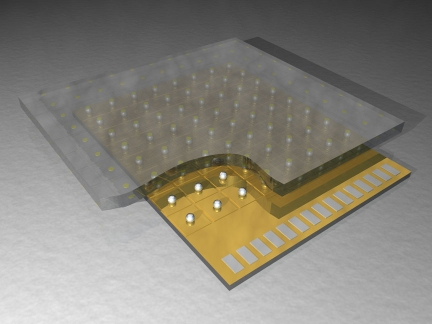
\includegraphics[width=0.47\textwidth]{bumpbonds}\label{pbumpbonds}}
	\hfill
	\subbottom[Photograph of an analogue pixel detector. The wire bonds are visible in the top right corner]{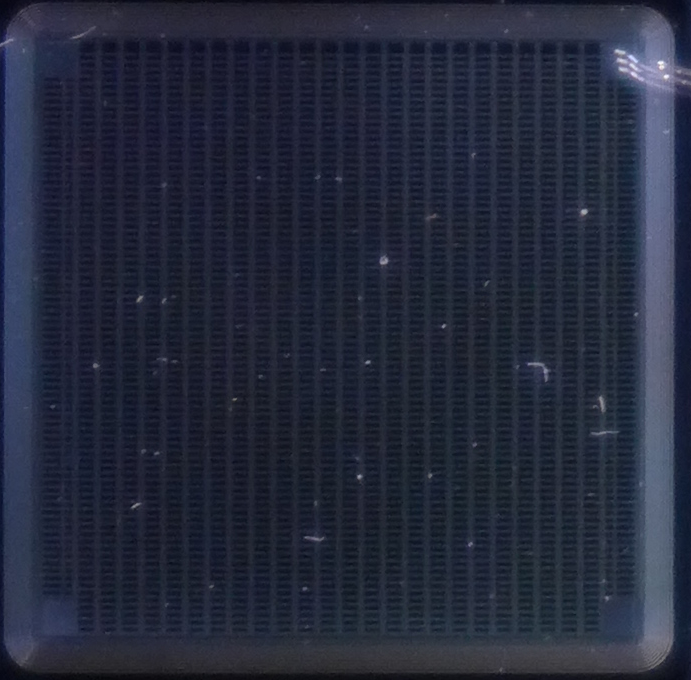
\includegraphics[width=0.47\textwidth]{ROC0}\label{p24}}
	\caption{Parts of the pixel detector.}
	\label{panaroc}
\end{figure}\no
% =======================
\subsection{Sensor}\label{s220}
For the current detector silicon is used as sensor material. The average energy to create an electron-hole pair in silicon is $3.6\,$eV. By applying a bias voltage to the sensor the charge carriers are moved to the collecting electrode and a signal can be measured. The silicon sensor itself consists of high-dose n-implanted pixels introduced into a high resistive n-substrate. The backside of the sensor is p-doped and thus creates a pn-junction \cite{allkofer}. The small pixel size was chosen to get a good spatial resolution. The thickness of the sensor is about $285\,\upmu$m so that minimum ionising particles will most probably create approximately $22000$ electron-hole pairs\footnote{The energy is loss is Landau distributed. This value is equivalent to the peak value of this distribution (q.v. \ar{slandau})} in the sensor. In order to fully deplete an unirradiated sensor of that thickness completely one has to apply a bias voltage of roughly $100\,$V \cite{pixadd}. For irradiated detectors that value may be a couple times higher, depending on the irradiation damage. 
% =======================
\subsection{\acs{ROC}}\label{sroc}
The \ac{ROC} has two parts: An active part consisting out of $26$ double columns of $2\times80$ \ac{PUC}s matching the pixels of the sensor and a periphery consisting of a control interface block, a data buffer, a time-stamp buffer and $35$ supply pads; this is depicted in \ar{p8}. All the signals going to and coming from the \ac{ROC} are put on these supply pads.\\
In order for the \ac{ROC} to record data, handle triggers and manage the readout, it also has four different counters:
\begin{enumerate}
	\item An $8\,$bit bunch crossing counter - whose information is sent to the time-stamp buffer,
	\item an $8\,$bit bunch crossing counter with trigger delay - runs a number of counts behind the bunch crossing counter (adjustable by the \ac{DAC} value wbc),
	\item an $4\,$bit trigger counter,
	\item an $4\,$bit token counter.
\end{enumerate}\par
The periphery is the reason is why the \ac{ROC} is with $7.9\,$mm$\times\ 9.8\,$mm a
\begin{wrapfigure}{l}{7.3cm}
	\vspace*{-10pt}
	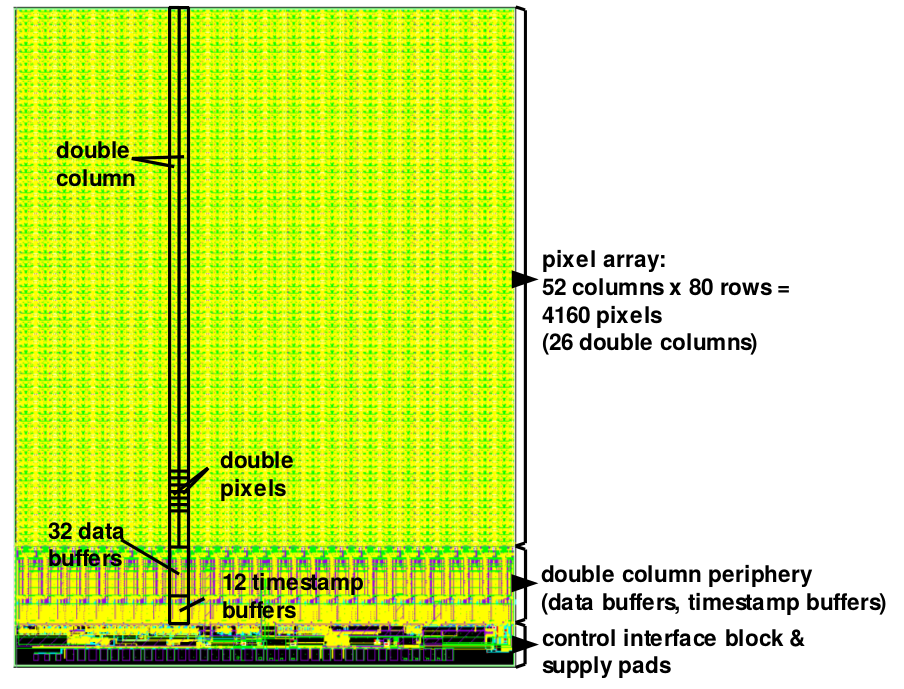
\includegraphics[width=7.2cm]{ROC_scheme}
	\caption{Schematics of a \ac{ROC} \cite{psi46chip}.}
	\label{p8}
	\vspace*{-5pt}
\end{wrapfigure}  
few millimetres longer than the pixelated area of the sensor. The \ac{ROC} is programmable with a set of  $26$ \ac{DAC} values (q.v. \ar{t0}) that are required to control its behaviour. More details about the \ac{DAC}s can be found in \ar{sdacs}. The \ac{ROC} and its behaviour is temperature dependent, which is why it is also equipped with a temperature sensor.\\
If electron-hole pairs are created in the sensor, a voltage signal is induced in the corresponding \ac{PUC}. A schematic of a \ac{PUC} is shown in \ar{p9}. Once a signal enters the \ac{PUC} it gets amplified and shaped. If it exceeds a certain threshold, which is tunable with one the \ac{DAC}s, a signal is immediately sent to the periphery that will save the current bunch crossing into the time stamp buffer. The information of the hit (the \ac{PUC} address and the \ac{PH}) will be sent to a sample and hold capacitance until it is read out, which happens every $25\,$ns. Once read out, the data is stored in the data buffer.\\ 
There is an option to sent calibration signals directly to the front end of the \ac{PUC} that makes it very easy to test the basic functionality of the \ac{ROC} without requiring any particle hits. For every pixel the \ac{PUC} has a register to enable and disable sending these calibrates.\\
Furthermore, an important feature of the analogue \ac{ROC} is the so called fast-OR. Every time the threshold of a single pixel is exceeded, the \ac{ROC} sends out this signal. It is an logical OR of all pixels of the \ac{ROC} and its shape gives, inter alia, conclusions about the distribution of hit pixels (q.v. \ar{sfastor}). It is very important as trigger signal for other devices or as self trigger.
\begin{figure}[ht]
	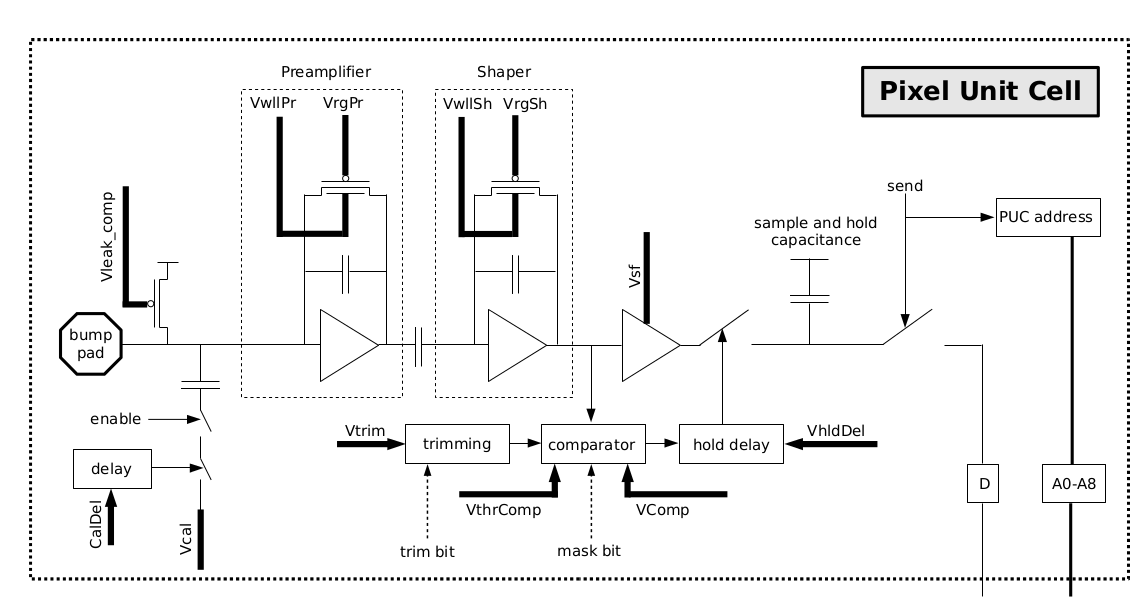
\includegraphics[width=0.95\textwidth]{PUC}
	\caption{Schematic view of a \ac{PUC} \cite{dambach}.}
	\label{p9}
\end{figure}
% =======================
\subsection{\acs{DAC}s}\label{sdacs}
An overview of all existing \ac{DAC}s for the analogue pixel chip with a short explanation is shown in \ar{t0} and \ar{t2}. In the following the most important \ac{DAC}s concerning this thesis are named.\\
In order to operate the chip it has to be supplied with a voltage. It was found that the chip is showing the best results while operating at a stable analogue current of $24\,$mA \cite{dambach}. This current can be adjusted by the $8\,$bit \ac{DAC} \textit{vana}. To be able to do basic tests with calibrate signals the correlation between \textit{vthrcomp} and \textit{caldel} has to be taken into account. It is only working in a certain region, which is explained in more detail in \ar{stornado}. Furthermore a common threshold for all pixels is of great importance. To achieve this a process called trimming is applied that exploits the inverse \ac{DAC} \textit{vthrcomp} and the \ac{DAC}s \textit{vcal} and \textit{vtrim}. More information about the trimming can be found in \ar{strim}. \textit{Vthrcomp} sets the global comparator threshold and \textit{vtrim} is responsible for the amount this global threshold can be lowered for each pixel. \textit{Vcal} regulates the amplitude of the calibrate signal and can be converted to the number of electrons created in the sensor. That is why it is also used to set a value for the common threshold.\\
Since for the undertaken experiments it was most important to have a stable fast-OR, \textit{vicolor}, \textit{vnpix} and \textit{vsumcol} were set in a way to have the maximum amplitude of the signal regardless of the shape. More details about the fast-OR and the effect of these \ac{DAC}s are in \ar{sfastor}.\\
\textit{Phoffset} and \textit{vcomp\_adc} can be used to adjust the address levels of the \ac{ROC}.
\begin{table}[ht]
	\begin{tabularx}{\textwidth}{c|l|X}
		\noalign{\hrule height 2pt}
		\textbf{\#} & \multicolumn{1}{c}{\textbf{Name(s)}} & \multicolumn{1}{|c}{\textbf{Explanation}}	\\\noalign{\hrule height 2pt}
		\multicolumn{3}{c}{\textbf{Voltage regulators}}														\\\hline
		$01$ & 	vdig				& sets the digital current 												\\\hline
		$02$ &	vana				& sets the analogue current 											\\\hline
		$03$ &  vsf // vsh			& influence on pulse height in low vcal range and digital current		\\\hline
		$04$ & 	vcomp				& regulates the supply voltage of the comparator						\\\noalign{\hrule height 2pt}
		\multicolumn{3}{c}{\textbf{Analogue Signal (\ac{PUC})}}												\\\hline
		$05$ &	vleak\_comp // vleak& controls leakage current 												\\\hline
		$06$ &	vrgpr				& \multirow{4}{7.6cm}{together control the pre-amplifier and the shaper and thereby the shape of the incoming signal}\\
		$07$ &	vwllpr				& 			 															\\
		$08$ &	vrgsh				& 																		\\
		$09$ &	vwllsh				&																		\\\hline
		$10$ &	vhlddel				& slightly influences the pulse height for different \textit{vcals} and pixels	\\\hline
		$11$ &	vtrim				& defines how much the trim bits for each pixel will increase the threshold\\\hline
		$12$ &	vthrcomp			& global comparator threshold											\\\noalign{\hrule height 2pt}
		\multicolumn{3}{c}{\textbf{Fast-OR Trigger (\ac{PUC})}}												\\\hline
		$22$ &	vicolor 			& \multirow{3}{7.6cm}{together define the shape of the fast-OR signal}		\\
		$23$ &	vnpix 				&  																		\\
		$24$ &	vsumcol	 			&  																		\\\noalign{\hrule height 2pt}
		\multicolumn{3}{c}{\textbf{Calibrate Signal (\ac{PUC})}}											\\\hline
		$22$ &	vcal	 			& sets the voltage for the calibrate signal (two ranges) 				\\\hline
		$22$ &	caldel	 			& delay of the calibrate signal											\\\noalign{\hrule height 2pt}
		\multicolumn{3}{c}{\textbf{Double Column Periphery}}												\\\hline
		$13$ &	vibias\_bus 		& switch for sending the address of the \ac{PUC} 						\\\hline
		$14$ &	vbias\_sf			& shifts the pulse height curve 										\\\hline
		$15$ &	voffsetop			& shift of pulse height  												\\\hline
		$16$ &	vibiasop			& switch for pulse height and influence of linear range 				\\\hline
		$17$ &	voffsetroc // phoffset	& switch for pulse height and influence of linear range 			\\\hline
		$18$ &	vion				& scaling of the pulse heights 											\\
		\noalign{\hrule height 2pt}
	\end{tabularx}					
	\caption{\ac{DAC}s of the pixel chip \cite{dambach}. Some \ac{DAC}s were renamed during the evolution of the chip which is why one \ac{DAC} can have several names.}
	\label{t0}
\end{table}\no
% =======================
\begin{table}[ht]
	\begin{tabularx}{\textwidth}{c|l|X}\noalign{\hrule height 2pt}
		\multicolumn{3}{c}{\textbf{Control and Interface Block}}											\\\hline
		$19$ &	ibias\_dac // vcomp\_adc	& scaling of the \ac{ROC} address levels and the pulse height 	\\\hline
		$20$ &	vibias\_ph // phscale& scaling of the pulse height 											\\\hline
		$21$ &	vibias\_roc 			& scaling of the \ac{ROC} address levels and the pulse height 		\\\noalign{\hrule height 2pt}
		\multicolumn{3}{c}{\textbf{Registers}}																\\\hline
		$253$ &	ctrlreg 			& switch between low and high vcal range (bit 2), full and half readout speed (bit 0) and on/off of the whole \ac{ROC} (bit 1)\\\hline
		$254$ &	wbc		 			& sets the bunch crossing at which the data will be read out 			\\\hline
		$255$ &	rangetemp 			& switch for different ranges of the temperature sensor  				\\\noalign{\hrule height 2pt}
	\end{tabularx}					
	\caption{\ac{DAC}s and Registers of the pixel chip \cite{dambach}}
	\label{t2}
\end{table}\no
% =======================
\subsection{Readout \& Trigger}\label{sread}
Each \ac{ROC} is set up to be read out in zero suppression mode, which means that only for pixel hits that exceed the threshold, the following information is sent to the periphery: The time stamp of the current bunch crossing is written into the time stamp buffer and the analogue signals are written into the next free data buffer. This process happens autonomously and asynchronously for every double column.\\
Concerning the readout of the \ac{ROC} two external signal lines are of importance: The \ac{CTR} and the token. As the name suggests, the former can send three kinds of information depending on the length of the pulse:
\begin{enumerate}
	\item a trigger signal, which is two clock cycles long.
	\item a calibrate signal, which is one clock cycle long.
	\item a reset signal, which is three clock cycle long.
\end{enumerate}
The information in the \ac{ROC} data buffer has to be kept until a potential trigger arrives. They are stored in the data buffer until one of the following events happens: 
\begin{itemize}
	\item The data was successfully read out by a connected device.
	\item The trigger window is exceeded (the bunch crossing counter passes the delayed time-stamp).
	\item The data buffer is full.
	\item A reset signal was received.
\end{itemize}
The process of the readout is described in the following: Hits that were sent to the periphery are validated by the external trigger signal by comparing their corresponding time stamps with the delayed bunch crossing counter. Non-validated hits are cleared. If the validation succeeds, the trigger counter is latched into the periphery, i.e. the double column is frozen and will not record further data until the information is read out or the \ac{ROC} receives a reset signal. Other double columns without validated hits remain active. When the latched trigger counter is matching the token counter the double column is set to readout mode and the trigger counter is incremented. As soon as the \ac{ROC} receives a token the frozen double columns are read out and reset. A token sent to the \ac{ROC} travels along the periphery consecutively reading out frozen \ac{DC}s. Just before the token leaves the periphery of a \ac{DC}, the token counter of that column is incremented as well. To every readout of the $26$ \ac{DC}s the \ac{ROC} also adds a header. Illustrations of the trigger validation and the readout procedure are shown in \ar{pro}.
\begin{figure}[ht]
	\centering
	\subbottom[Trigger validation.]{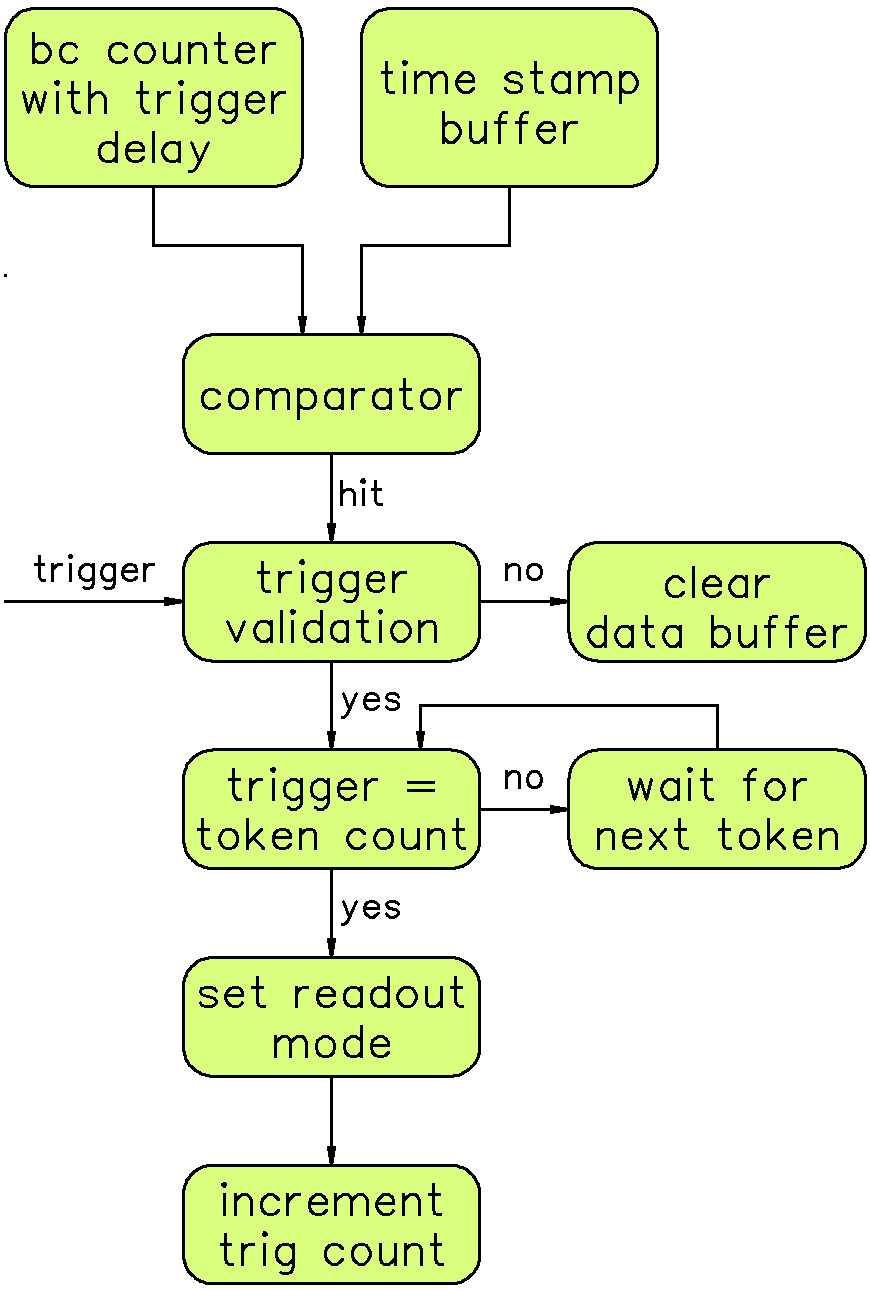
\includegraphics[width=0.37\textwidth]{trigger}\label{ptrig}}
	\hfill
	\subbottom[Readout procedure.]{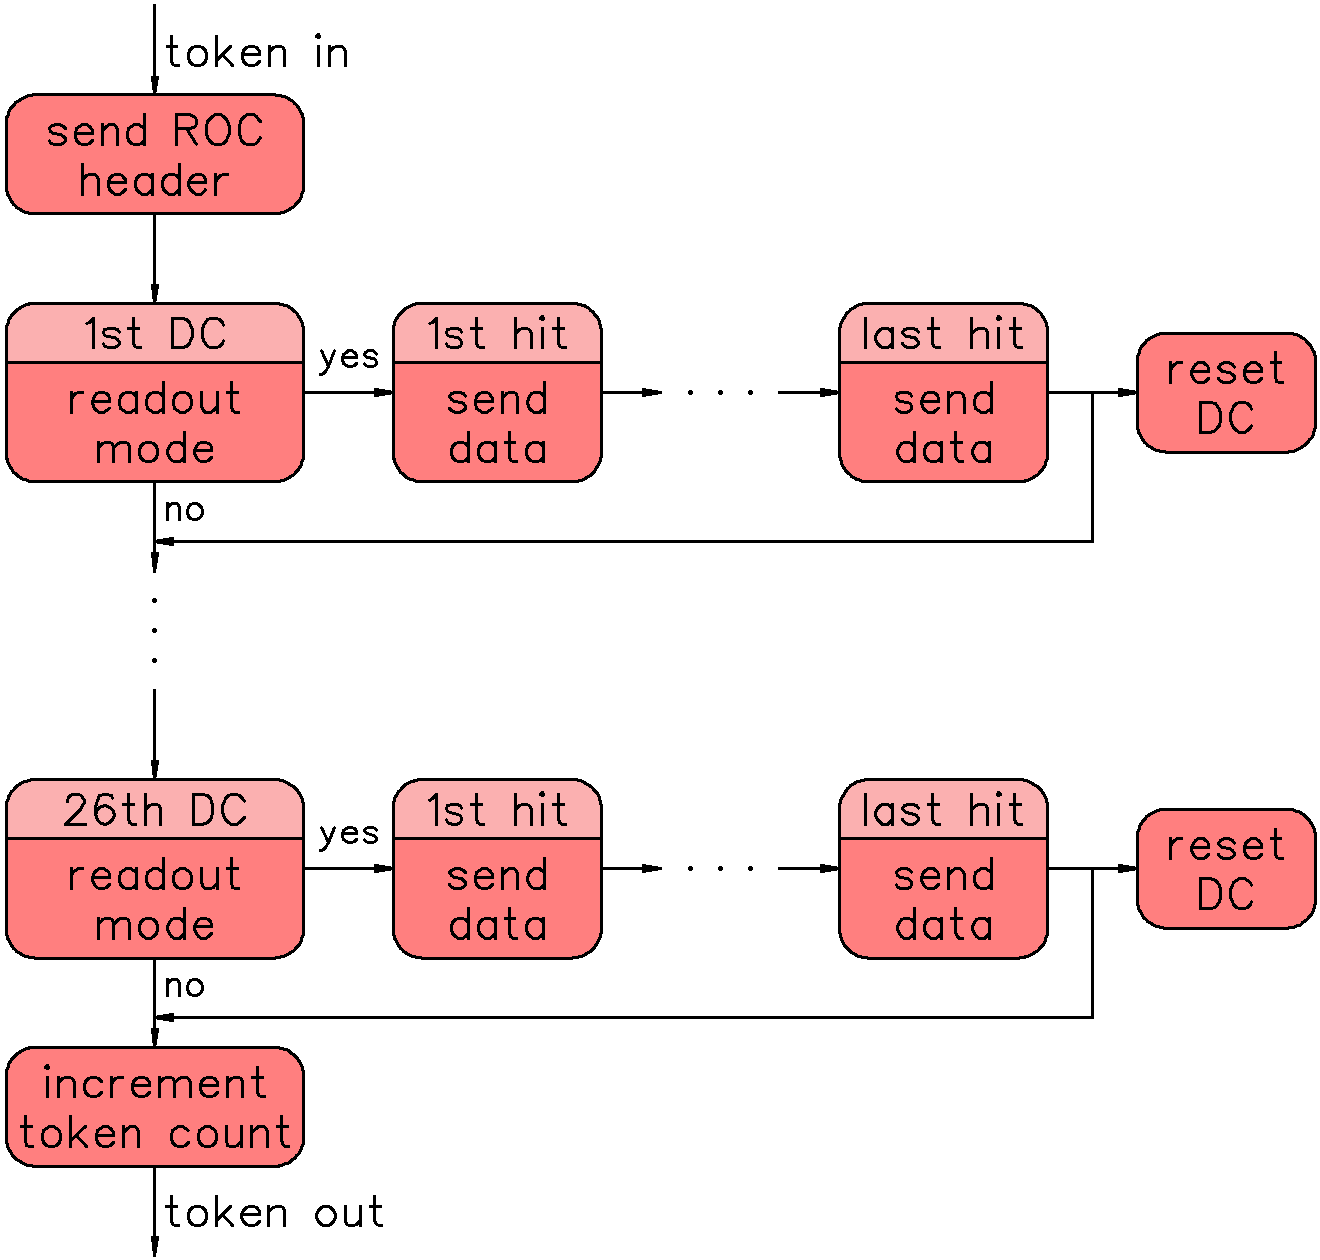
\includegraphics[width=0.57\textwidth]{token}\label{ptok}}
	\caption{Schematics of the readout of the \ac{ROC}. bc is short for bunch crossing and DC stands for double column}
	\label{pro}
\end{figure}\no
% =======================
\subsection{Data Format}\label{sdata}
An example of an analogue readout with only the information of the \ac{ROC} is shown in \ar{procsig}. The \ac{ROC} header is three clock cycles long. It contains an \ac{UB} level that is a very low, negative level and serves as reference, a \ac{B} level that is the zero reference of the differential signal and a level that is called \ac{LD}. The latter either points to the value the last \ac{DAC} was set to or the value of the temperature sensor of the chip. For every single pixel that was hit the \ac{ROC} will provide five levels containing the pixel address and one level with information about the pulse height. These six level are added to the header for each hit pixel. If no pixel was hit or the hits were not validated, the \ac{ROC} will send nothing but a header if a readout is started.\\
It is possible to read out several \ac{ROC}s with a single token. In that case the token is sent from one \ac{ROC} to the next collecting a header of each \ac{ROC} and the corresponding hit information s.t. a structure like header/hit/header/hit/hit/header/header/hit etc. will form. The readout concerning sending and handling trigger, reset and token is managed by a \ac{TBM}. For all the experiments described in the thesis the data was read with a \ac{DTB} that was developed at \ac{PSI}. The \ac{DTB} utilises a \ac{TBM} emulated on its \ac{FPGA} and is described in more detail in \ar{sdtb}.\\
\begin{figure}[ht]
	\centering
	\subbottom[Measured signal of several single pixel hits.\label{panasig}]{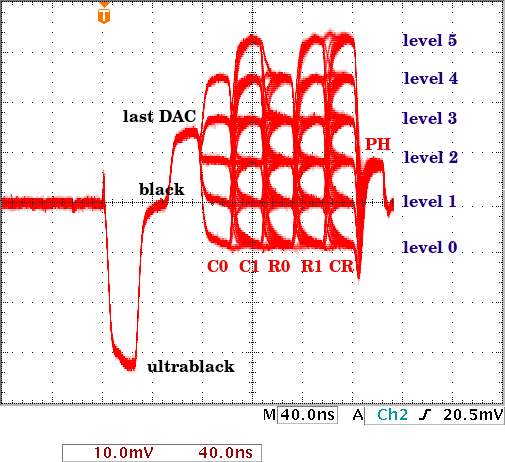
\includegraphics[width=0.47\textwidth]{siganalog}}
	\hfill
	\subbottom[Schematic signal of one single pixel hit.\label{p7}]{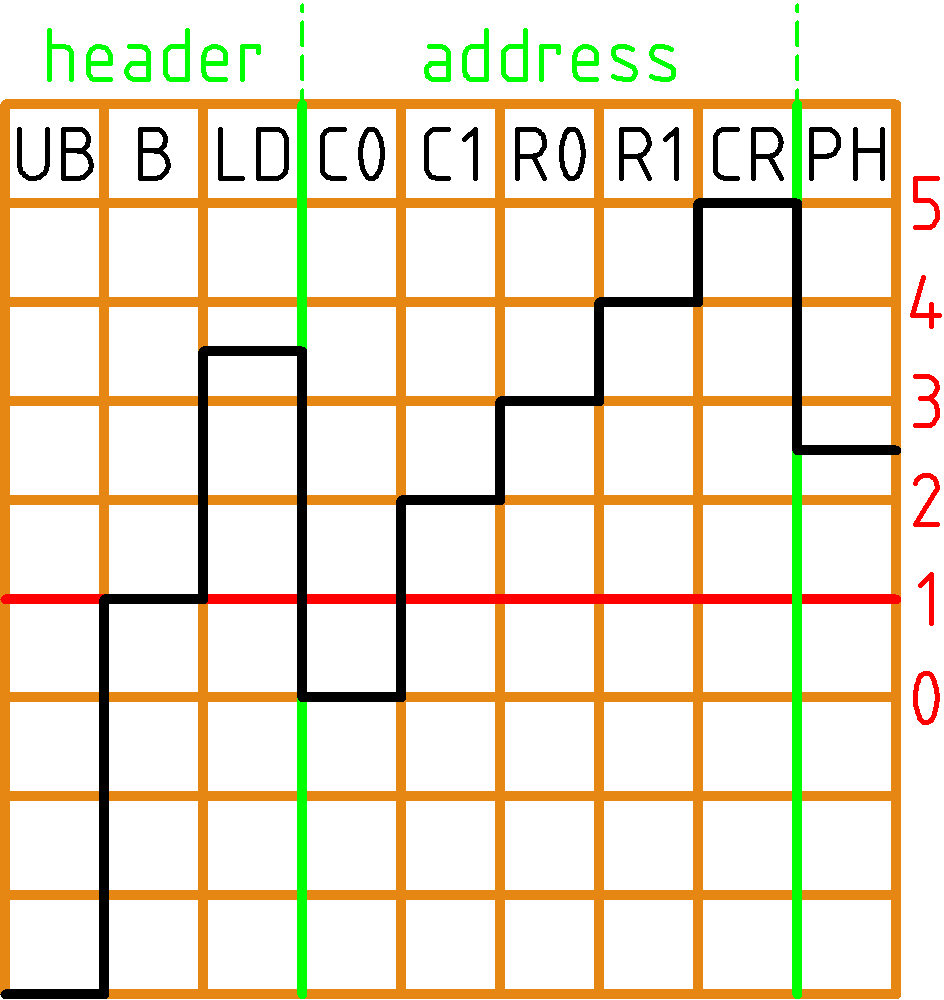
\includegraphics[width=0.47\textwidth]{levels}}
	\caption{Signals of the analogue \ac{ROC}}
	\label{procsig}
\end{figure}\no
% =======================
\subsubsection{\ac{I2C} Address}\label{si2c}
In order to be able to operate more than one \ac{ROC} with a single \ac{DTB}, every \ac{ROC} has a $4\,$bit \ac{I2C} address. The address can be set by connecting the supply pads $22-25$ to ground, of which each is equivalent to one bit. The bits are active if they are grounded, therefore the \ac{I2C} address is zero if none of the pads is connected. By sending commands to these addresses each \ac{ROC} can be programmed independently.
% =======================
\subsubsection{\ac{TBM}}\label{stbm}
\begin{figure}[ht]
	\centering
	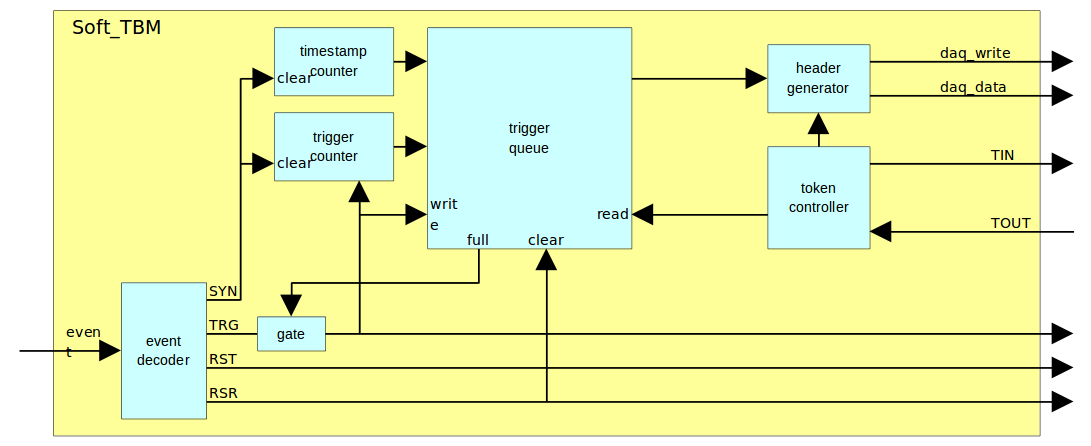
\includegraphics[width=0.95\textwidth]{tbm}
	\caption{Process chart of the emulated \ac{TBM}.}
	\label{ptbm}
\end{figure}\no
A process chart of the basic functionality of the \ac{DTB}'s \ac{TBM} is shown in \ar{ptbm}. While passing through the \ac{TBM} incoming triggers [TRG]  increment the $4./$bit trigger counter and write an entry into the trigger queue. This information is then read by the token controller, which sends out a token [TOUT] for each trigger and also receives the tokens [TIN] again that went to the \ac{ROC}. Once the token was received the the respective trigger gets cleared from the queue. The maximum amount of triggers in the trigger queue is $16$. If more triggers pile up until the [TIN] comes back, the triggers are caught by a gate where they are annihilated. There is also the possibility to clear the trigger queue with a reset signal. The token controller as well as the trigger queue send information to the header generator. When [TIN] arrives the header generator adds the information to the digital data stream in form of a header and a trailer, which each consist of two $16\,$ bit data words. The header contains an $8\,$bit event number and information about the trigger position inside the clock cycle.  The trailer contains, inter alia, a stack counter that is equivalent to the number of queued triggers. More information about the header and the trailer of the \ac{TBM} are given in \ar{stbmprob}. 
% ========================================================
\section{Digital Pixel Detector}\label{s23}
\begin{wrapfigure}{r}{4.5cm}
	\vspace*{-10pt}
	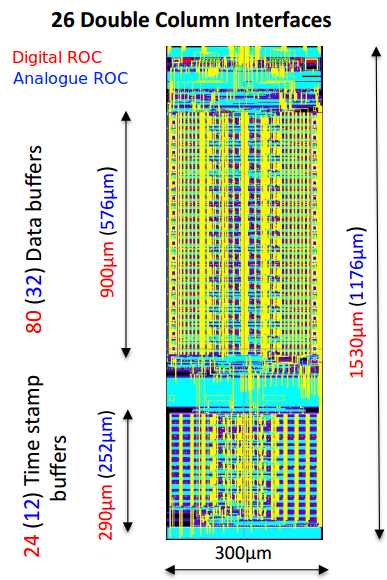
\includegraphics[width=4.4cm]{DigRocPeri}
	\caption{Double column interface of the digital \ac{ROC} \cite{hits}}
	\label{p12}
	\vspace*{-15pt}
\end{wrapfigure} 
For the Phase 1 Upgrade of \ac{CMS} a new digital \ac{ROC} was designed based on the analogue one. Their functionality is in principle still the same. An overview of the differences can be found in \ar{t3}.\\
One of the limitation of the analogue \ac{ROC} was a limited buffer size for the Level 1 trigger latency. To overcome this problem the number of data buffers was increased from $32$ to $80$. To reduce the readout related dead times due to higher rate, the number of time stamp buffers was doubled from $12$ to $24$. In addition the readout bandwidth had to be increased. This was done by switching to a fully digital readout by means of an on-chip \ac{ADC} for every \ac{DC}, new fast digital readout links, a \ac{PLL} to provide higher frequencies and some modifications to the control logic.An important feature of the new is the lower overall signal threshold that also increases the persistence of the chip \cite{hits}. This feature is indispensable for the low signals of diamonds, which is a possible candidate for a new generation of pixel chips. Going to lower thresholds was achieved by keeping the timewalk between the highest and lowest signal amplitudes within one clock cycle ($<16\,$ns) and reducing the cross talk in the digital \ac{ROC} layout as well as lower electronic noise. Besides, the output of the fast-Or signal was removed from the digital \ac{ROC}.\\
For easier usage the number of \ac{DAC} parameters is reduced to $16$. There is now only one parameter (\textit{vwllpr} and \textit{vwllsh}) for the pre-amplifier and the shaper instead of two and the leakage current compensation was removed. The six \ac{DAC}s for the double column periphery, which are responsible for the shape of the pulse height vs. \textit{vcal} curve, were condensed into \textit{vibias\_bus} and \textit{phoffset}. A comparison of the \ac{DAC}s that changed can be found in \ar{tdacchange}.
\begin{table}[ht]
	\centering
	\begin{tabularx}{0.85\textwidth}{X|l|l}\noalign{\hrule height 2pt}
			 &\multicolumn{1}{c}{\textbf{psi46v2}}	&\multicolumn{1}{|c}{\textbf{psi46dig}}	\\\hline
		\ac{ROC} size					& $7.9\times9.8\,$mm	& $7.9\times10.2\,$mm 	\\
		Pixel size						& $100\times150\,\upmu$m& $100\times150\,\upmu$m\\
		Smallest radius					& $4.3\,$cm				& $2.9\,$cm				\\
		\ac{DAC}s / registers			& $26$ / $3$			& $16$ / $3$			\\
		Power up condition				& not defined			& default values		\\
		Pixel charge readout			& analogue				& digitised, $8\,$bit	\\
		Readout speed					& $40\,$MHz				& $160\,$Mbit/s			\\
		Time stamp buffer size			& $12$					& $24$					\\
		Data buffer size				& $32$					& $80$					\\
		Output buffer FIFO				& no					& yes					\\
		Double column speed				& $20\,$MHz				& $40\,$MHz				\\
		Metal layers					& $5$					& $6$					\\
		leakage current compensation	& yes					& no					\\
		In-time threshold				& $3500\,$e				& $<2000\,$e			\\
		\ac{PLL}						& no					& yes					\\
		Data loss at max 				& $\sim3.8\,$\% at  	& $\sim3\,$\% at		\\
		operating flux					& $120\,$Mhz/cm$^{2}$	& $580\,$Mhz/cm$^{2}$ \footnotemark[2]\\\noalign{\hrule height 2pt}
	\end{tabularx}					
	\caption{comparison between analogue and digital \ac{ROC} \cite{hits}}
	\label{t3}
\end{table}\no
\footnotetext[2]{This is valid for the layer 1 version of the digital chip, that is planned for the Phase 1 Upgrade.}
\begin{table}[ht]
	\begin{tabularx}{\textwidth}{c|l|l|X}
		\noalign{\hrule height 2pt}
		\textbf{\#} & \multicolumn{1}{l}{\textbf{analogue}} & \multicolumn{1}{|l}{\textbf{digital}}	& \multicolumn{1}{|l}{\textbf{comment}}\\\noalign{\hrule height 2pt}
		\multicolumn{4}{c}{\textbf{Analogue Signal (\ac{PUC})}}							\\\hline
		$05$ &	vleak				& $-$ 		& leakage current compensation removed			\\
		$06$ &	vrgpr				& $-$ 		& combined into vwllpr		\\	
		$07$ &	vwllpr				& vwllpr	&							\\
		$08$ &	vrgsh				& $-$		& combined into vwllsh		\\
		$09$ &	vwllsh				& vwllsh	&							\\\noalign{\hrule height 2pt}
		\multicolumn{4}{c}{\textbf{Double Column Periphery}}				\\\hline
		$13$ &	vibias\_bus 		& vibias\_bus	&						\\
		$14$ &	vbias\_sf			& $-$			&						\\
		$15$ &	voffsetop			& $-$			& the six periphery dacs\\
		$16$ &	vibiasop			& $-$			& were condensed into two \\
		$17$ &	voffsetroc			& phoffset		& 						\\
		$18$ &	vion				& $-$			&						\\\noalign{\hrule height 2pt}
		\multicolumn{4}{c}{\textbf{Control and Interface Block}}			\\\hline
		$19$ &	vibias\_dac 		& vcomp\_adc 	&						\\
		$20$ &	vibias\_ph 			& phscale 		& 						\\
		$21$ &	vibias\_roc 		& $-$			& removed				\\\noalign{\hrule height 2pt}
		\multicolumn{4}{c}{\textbf{Fast-OR Trigger (\ac{PUC})}}				\\\hline
		$22$ &	vicolor 			& vicolor	&							\\
		$23$ &	vnpix 				& $-$		& fast-OR removed			\\
		$24$ &	vsumcol	 			& $-$		& fast-OR removed			\\
		\noalign{\hrule height 2pt}
	\end{tabularx}					
	\caption{Different \ac{DAC}s for analogue and digital \ac{ROC}}
	\label{tdacchange}
\end{table}\no
% ========================================================
\section{Digital Test Board}\label{sdtb}
The psi46 \ac{DTB} is the interconnect between a computer and the \ac{ROC}. In the past the analogue chips were operated with an \ac{ATB}, which has some major disadvantages in comparison with the \ac{DTB}. For example it has only a limited amount of data it can save, s.t. during beam tests one could only take runs of $300000$ events until the buffer was full. One of the achievements of this thesis is the possibility to reliably operate analogue chips as well as digital chips with the \ac{DTB}.\\
The \ac{DTB} is powered by a $6\,$V AC to DC power supply and connects via an adapter to the \ac{ROC}. It has two interfaces to a computer of which the ethernet is not implemented yet, leaving the USB 2.0 as only option. In here lies another advantage compared to the \ac{ATB}, which only had a USB 1.1 connection: The writing speed is increased a lot. In order to use several \ac{DTB}s on the same computer, each \ac{DTB} has its own serial number. Once connected to the chip and a computer, the \ac{DTB} and its \ac{FPGA} are completely controlled with a software called pXar. The \ac{FPGA}, which is emulating the \ac{TBM}, has its own firmware developed at \ac{PSI}. By now there more than twenty iterations of this firmware, which can be easily upgraded via USB. During this thesis the firmware versions from $4.0$ to $4.2$ were utilised.\\
It is possible to read out several signals of the \ac{DTB}. For that purpose there are two digital and two differential analogue LEMO outputs.\\
Furthermore the \ac{DTB} has inputs for an external clock and trigger, which accept \ac{TTL} signals. The height of the external trigger signal has to be at least $3\,$V to guarantee stability. Since these inputs are not terminated, it is very important to terminate incoming signals at the input to avoid reflections inside the cables. The \ac{DTB} also has a \ac{HV} input that is able to distribute the \ac{HV} to the sensor.
\begin{figure}[ht]
	\centering
	\subbottom[Top view.]{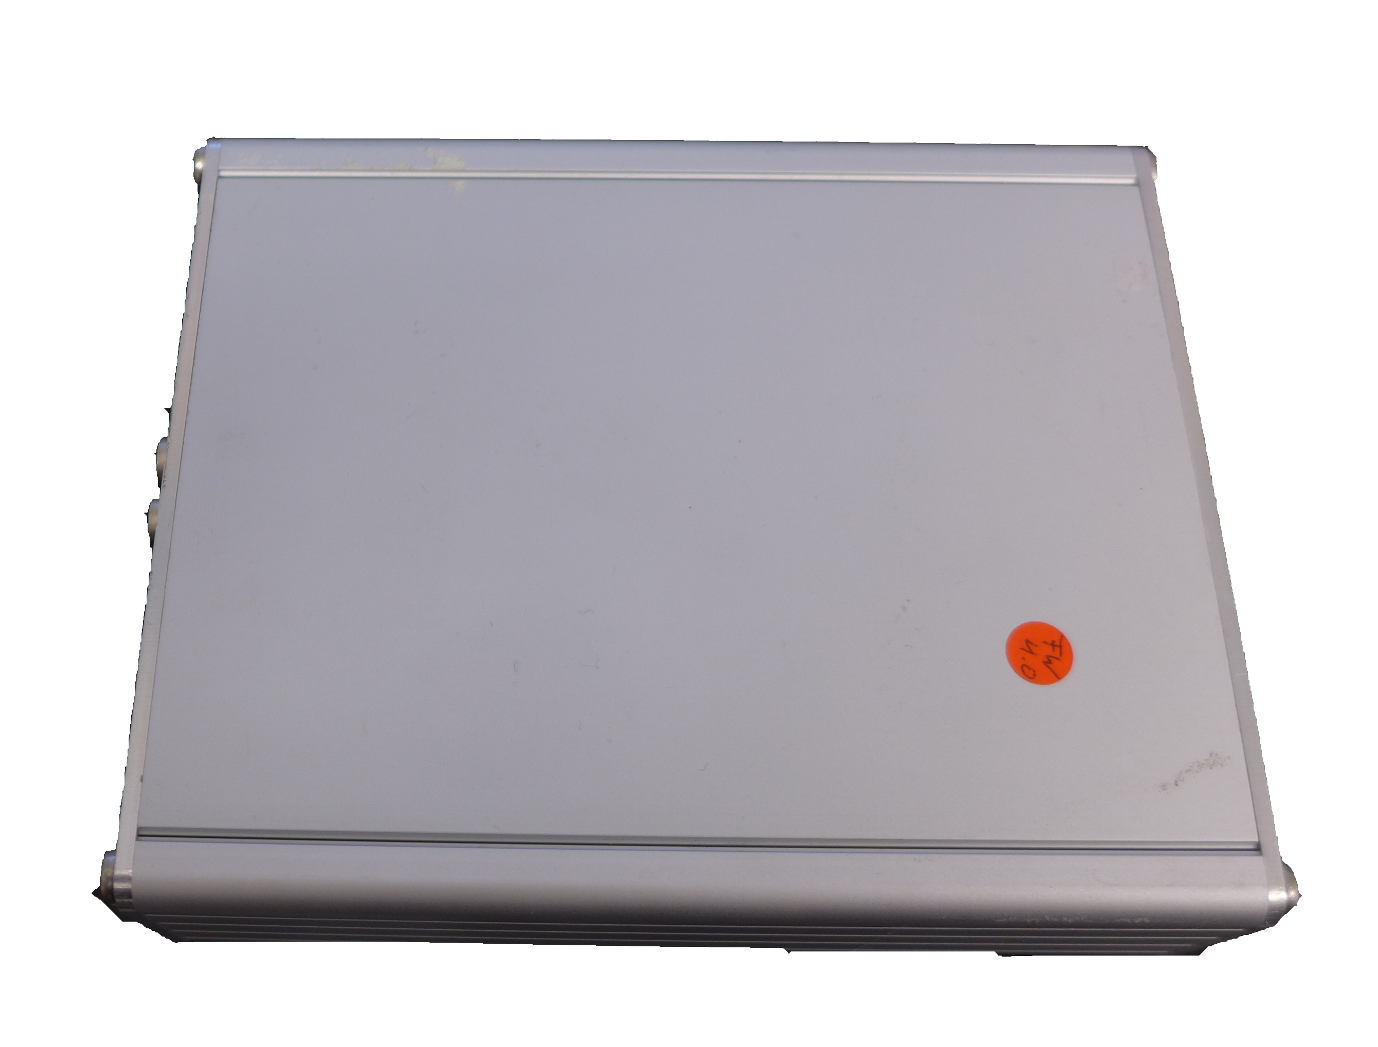
\includegraphics[width=0.47\textwidth]{DTB}\label{p10}}
	\hfill
	\subbottom[Front and backside.]{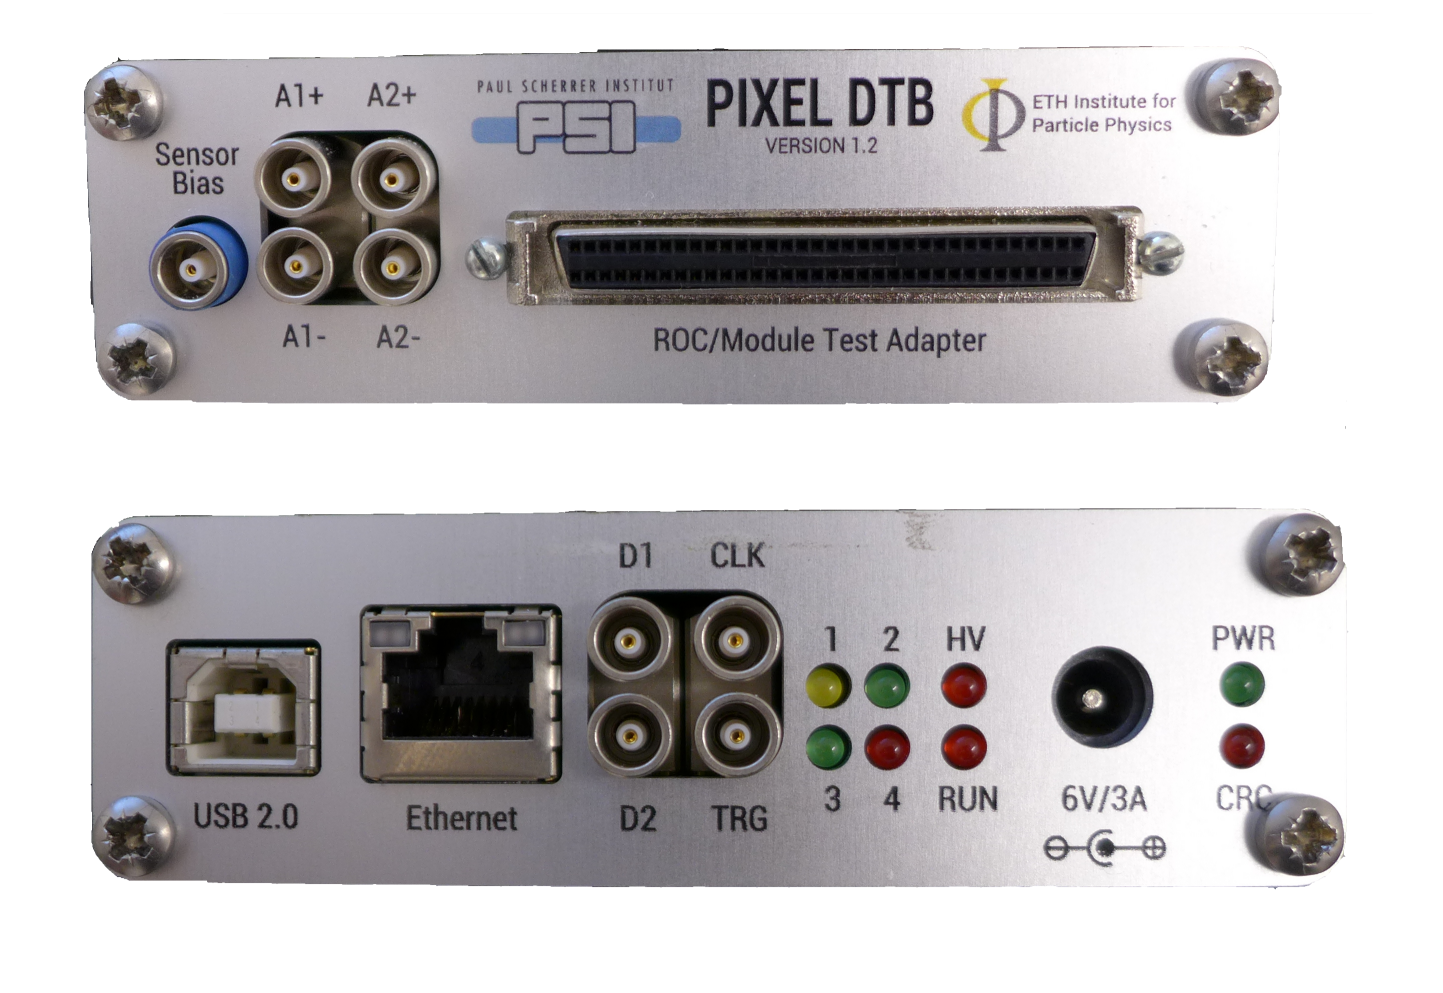
\includegraphics[width=0.47\textwidth]{DTB-Sides}\label{p11}}
	\caption{Photographs of the \ac{DTB}.}
	\label{pdtb}
\end{figure}\no
% ========================================================
% TO GET IT COMPILED
% ========================================================
\chapter*{List of Acronyms}
\begin{acronym}[Bash]
	\acro{PUC}{pixel unit cell}
	\acro{ROC}{readout chip}
	\acro{TBM}{token bit manager}
	\acro{UB}{ultra black}
	\acro{B}{black}
	\acro{CMS}{Compact Muon Solenoid}
	\acro{LHC}{Large Hadron Collider}
	\acro{CERN}{European Organization for Nuclear Research}
	\acro{DAC}{digital to analogue converter}
	\acro{ADC}{analogue to digital converter}
	\acro{LD}{last DAC}
	\acro{DTB}{digital test board}
	\acro{ATB}{analogue test board}
	\acro{ETH}{Eidgen{\"o}ssische Technische Hochschule}
	\acro{FPGA}{Field Programmable Gate Array}
	\acro{PSI}{Paul Scherrer Institut}
	\acro{HV}{high voltage}
	\acro{TTL}{Transistor-Transistor-Logic}
	\acro{PLL}{phase-locked loop}
	\acro{FIFO}{First In - First Out}
	\acro{HAL}{hardware abstraction layer}
	\acro{API}{application programming interface}
	\acro{GUI}{graphical user interface}
	\acro{CLI}{command line interface}
	\acro{DAQ}{data acquisition}
	\acro{CPU}{central processing unit}
	\acro{PG}{pattern generator}
	\acro{I2C}[I$^{2}$C]{Inter-Integrated Circuit}
	\acro{DUT}{device under test}
	\acro{TCP}{Transmission Control Protocol}
	\acro{TU}{trigger unit}
	\acro{COM}{centre of mass}
	\acro{PSB}{Proton Synchrotron Booster}
	\acro{PS}{Proton Synchrotron}
	\acro{SPS}{Super Proton Synchrotron}
	\acro{ALICE}{A Large Ion Collider Experiment}
	\acro{ATLAS}{A Toroidal LHC Apparatus}
	\acro{LHCb}{Large Hadron Collider beauty}
	\acro{LHCf}{ Large Hadron Collider forward}
	\acro{TOTEM}{TOTal Elastic and diffractive cross section Measurement}
	\acro{SUSY}{supersymmetry}
	\acro{HCAL}{hadronic calorimeter}
	\acro{ECAL}{electromagnetic calorimeter}
	\acro{CTR}{calibrate trigger reset}
	\acro{MIP}{minimum ionising particle}
	\acro{PM}{photo multiplier}
	\acro{TLU}{trigger logic unit}
	\acro{PH}{pulse height}
	\acro{DC}{double column}
	\acro{DESY}{Deutsches Elektronen-Synchrotron}
	\acro{RAM}{Random-Access Memory}
	\acro{PCB}{printed circuit board}
	\acro{PLT}{Photo Luminosity Telescope}
	\acro{RPC}{remote procedure calls}
\end{acronym}
\bibliographystyle{plain}
\bibliography{refs}
\end{document}